\documentclass[conference]{IEEEtran}
\usepackage{cite}
\usepackage{amsmath,amssymb,amsfonts}
\usepackage{algorithmic}
\usepackage{graphicx}
\usepackage{textcomp}
\usepackage{xcolor}
\usepackage[indonesian]{babel}
\addto\captionsindonesian{\renewcommand{\abstractname}{Abstrak}\renewcommand{\refname}{Daftar Pustaka}}
\renewcommand{\IEEEkeywordsname}{Kata Kunci}
\graphicspath{{figures/}}

\begin{document}

\title{Analisis Trade-off antara Akurasi dan Efisiensi Komputasi dalam Deteksi Sarkasme Menggunakan DistilBERT dan RoBERTa}

\author{\IEEEauthorblockN{Falah Razan Hibrizi}
\IEEEauthorblockA{\textit{Fakultas Informatika} \\
\textit{Universitas Telkom}\\
Bandung, Indonesia \\
alamat email}
\and
\IEEEauthorblockN{Nama Pembimbing}
\IEEEauthorblockA{\textit{Fakultas Informatika} \\
\textit{Universitas Telkom}\\
Bandung, Indonesia \\
alamat email}
}

\maketitle

\begin{abstract}
\end{abstract}

\begin{IEEEkeywords}
\end{IEEEkeywords}

\section{Pendahuluan}

\section{Metode}
Penelitian ini membandingkan performa dan efisiensi komputasi RoBERTa dan DistilBERT, lalu melihat trade-off di antara keduanya. Perbandingan tersebut dijabarkan melalui tiga pertanyaan penelitian, yaitu apakah jumlah layer yang dibekukan berpengaruh terhadap performa klasifikasi sarkasme, apakah parent comment sebagai input berpengaruh terhadap performa tersebut, dan strategi fusion mana yang memberikan performa terbaik. Ketiga pertanyaan dijawab untuk kedua model beserta biaya komputasinya.

\subsection{Dataset dan Prapemrosesan}
Data yang digunakan adalah versi seimbang Self-Annotated Reddit Corpus (SARC) \cite{khodak2018sarc} dari rilis Kaggle yang juga dipakai pada \cite{dubey2026efficient} dan \cite{zhang2025enhancing}. Data ini berisi 1.010.826 pasangan comment Reddit dan parent comment yang dibalasnya. Label tidak dibuat oleh anotator; sebuah comment dianggap sarkas apabila penulisnya menandainya dengan ``/s'', dan penanda ini dihapus dari teks saat korpus disusun \cite{khodak2018sarc}.

Prapemrosesan dibuat ringan. Penelitian sebelumnya mengubah teks menjadi huruf kecil, menghapus tanda baca atau karakter khusus, dan melakukan lematisasi \cite{dubey2026efficient}, \cite{zhang2025enhancing}. Langkah tersebut tidak dilakukan di sini karena huruf kapital, tanda baca, dan emotikon seperti ``;)'' dapat menjadi penanda sarkasme. Pembersihan hanya mendekode entitas HTML, mengganti tautan Markdown dengan teksnya, menghapus URL dan tag HTML, serta merapikan spasi, sehingga hanya 2.942 comment (0,29\%) yang berubah.

Tabel~\ref{tab:data} menunjukkan baris yang dibuang pada setiap tahap. Duplikat dan label yang bertentangan dicari dengan kunci yang dinormalisasi (huruf kecil, tanpa tanda baca), tetapi model tetap menerima teks asli. Tahap terakhir membuang artefak dari penghapusan penanda ``/s'', yaitu comment yang hanya berisi potongan kalimat seperti ``You forgot the''. Potongan ini dideteksi dengan pola maksimal delapan kata, dan 8.580 dari 8.599 baris yang cocok berlabel sarkas, sehingga baris tersebut dibuang agar model tidak memakai jalan pintas. Data akhir berisi 1.000.864 pasangan dengan 49,59\% sarkas.

\begin{table}[t]
\caption{Penyaringan Baris dan Pembagian Data}
\label{tab:data}
\centering
\begin{tabular}{lrr}
\hline
Tahap penyaringan & Dibuang & Sisa \\
\hline
Data mentah & -- & 1.010.826 \\
Comment kosong & 55 & 1.010.771 \\
Kosong setelah dibersihkan & 9 & 1.010.762 \\
Label bertentangan & 142 & 1.010.620 \\
Pasangan duplikat & 1.157 & 1.009.463 \\
Potongan ``/s'' & 8.599 & 1.000.864 \\
\hline
Bagian data & Pasangan & Sarkas (\%) \\
\hline
Latih & 799.459 & 49,66 \\
Validasi & 100.276 & 49,38 \\
Uji & 101.129 & 49,27 \\
\hline
\end{tabular}
\end{table}

Data dibagi menjadi data latih, validasi, dan uji dengan seed 42. Pembagian dilakukan per kelompok comment, bukan per baris, sehingga comment dengan kunci yang sama selalu berada di bagian yang sama. Hal ini penting karena balasan pendek seperti ``Source?'' dan ``Yes.'' muncul ratusan kali. Proporsinya mendekati 80/10/10, dan tidak ada comment atau pasangan yang muncul di lebih dari satu bagian.

\subsection{Model dan Konfigurasi Input}
RoBERTa-base \cite{liu2019roberta} memiliki 12 layer Transformer, ukuran hidden 768, dan 124,6 juta parameter. DistilBERT \cite{sanh2019distilbert} adalah hasil distilasi BERT dengan ukuran hidden yang sama, tetapi hanya enam layer dan 65,8 juta parameter. Versi cased dari DistilBERT digunakan agar kedua model sama-sama menerima huruf kapital. Tiga konfigurasi input dibandingkan untuk melihat pengaruh parent comment dan strategi fusion.

\textit{Comment saja.} Model hanya membaca balasan, dan konfigurasi ini menjadi baseline.

\textit{Early fusion.} Parent dan comment digabung menjadi satu input dengan format pasangan kalimat dari tokenizer, dengan parent di depan, seperti penggabungan konteks dan respons pada \cite{ataeii2020transformers}. Setiap token comment dapat memperhatikan seluruh token parent sejak layer pertama. Panjang input dibatasi 256 token, dan bila lebih panjang, bagian akhir parent dipotong (0,85\% pasangan latih pada RoBERTa dan 0,99\% pada DistilBERT).

\textit{Late fusion.} Parent dan comment di-encode terpisah oleh encoder yang sama. Hidden state akhir token pertama comment ($h_x$) dan parent ($h_y$) digabung menjadi
\begin{equation}
u = [\,h_x;\; h_y;\; |h_x - h_y|;\; h_x \odot h_y\,],
\label{eq:fusion}
\end{equation}
dengan $[\cdot\,;\cdot]$ menyatakan penggabungan vektor dan $\odot$ perkalian per elemen. Vektor $u$ pada (\ref{eq:fusion}) masuk ke head klasifikasi yang strukturnya mengikuti head bawaan setiap model, tetapi dengan input empat kali lebih lebar. Pemotongan teks mengikuti early fusion. Konsekuensinya, encoder dijalankan dua kali per contoh dan parent tidak saling memperhatikan dengan comment.

\subsection{Pembekuan Layer}
Untuk melihat pengaruh pembekuan layer, embedding layer dan sejumlah layer terbawah dibekukan sehingga hanya layer atas dan head yang dilatih. Pembekuan diuji pada early fusion, yaitu 0, 6, 9, dan 12 dari 12 layer RoBERTa serta 0, 3, dan 6 dari 6 layer DistilBERT. Model yang dibekukan sebagian dilatih dengan tiga seed dan learning rate terbaik dari fine-tuning penuh. Model yang seluruh layernya dibekukan dilatih dengan learning rate $10^{-4}$ dan $10^{-3}$ pada seed 42 saja, lalu dipilih yang terbaik pada data validasi. Pembekuan hanya mengurangi biaya training, karena semua layer tetap dijalankan saat inferensi.

\subsection{Pengaturan Eksperimen}
Tabel~\ref{tab:setup} merangkum pengaturan training. Weight decay tidak diterapkan pada bias dan parameter LayerNorm, dan setiap batch hanya di-padding sampai urutan terpanjangnya. Epoch dengan macro-F1 validasi tertinggi yang dipilih. Learning rate dicari sendiri karena RoBERTa diketahui sensitif terhadap pengaturan training \cite{jimenez2026bert}, dengan grid yang mencakup nilai $2 \times 10^{-5}$ dan $3 \times 10^{-5}$ dari \cite{dubey2026efficient}, \cite{ullah2026advanced}.

\begin{table}[t]
\caption{Pengaturan Training}
\label{tab:setup}
\centering
\begin{tabular}{ll}
\hline
Pengaturan & Nilai \\
\hline
Panjang input maksimum & 256 token \\
Ukuran batch & 32 (evaluasi: 128) \\
Epoch & maks. 3, terbaik menurut macro-F1 validasi \\
Loss & cross-entropy \\
Optimizer & AdamW, weight decay 0,01 \\
Jadwal learning rate & warm-up linear 10\%, lalu turun linear \\
Gradient clipping & 1,0 \\
Dropout classifier & 0,1 (RoBERTa), 0,2 (DistilBERT) \\
Presisi & BF16 mixed precision \\
Grid learning rate (S1) & $\{1, 2, 3, 5\} \times 10^{-5}$ \\
Seed & 42 (S1); 42, 43, 44 (run final) \\
\hline
\multicolumn{2}{l}{Learning rate terpilih (RoBERTa / DistilBERT)} \\
\quad Comment saja & $1 \times 10^{-5}$ / $3 \times 10^{-5}$ \\
\quad Early fusion & $2 \times 10^{-5}$ / $1 \times 10^{-5}$ \\
\quad Late fusion & $1 \times 10^{-5}$ / $1 \times 10^{-5}$ \\
\hline
\end{tabular}
\end{table}

Sebanyak 60 run dijalankan dalam tiga skenario: pencarian learning rate dengan seed 42 (S1, 24 run), pembekuan layer (S2, 16 run), dan pengulangan konfigurasi terpilih dengan seed 43 dan 44 (S3, 20 run). Semua run memakai satu GPU NVIDIA GeForce RTX 5070 Ti 16 GB. Waktu training diukur per epoch tanpa validasi, dan memori adalah memori GPU puncak selama training. Latensi adalah waktu forward pass dengan input yang sudah berada di GPU, diukur pada 1.000 contoh validasi untuk ukuran batch 1 dan 32 dan dilaporkan per contoh. Angka efisiensi dirata-ratakan dari run final yang sama dengan skor data uji.

\subsection{Evaluasi dan Uji Statistik}
\label{sec:eval}
Comment diprediksi sarkas apabila probabilitasnya minimal 0,5. Metrik yang dilaporkan adalah accuracy, precision, recall, dan F1 kelas sarkas, serta macro-F1 sebagai metrik utama. Epoch dan learning rate hanya dipilih dengan data validasi. Prediksi data uji disimpan tanpa dinilai, dan 29 run final dicatat dalam file manifest yang di-commit ke repositori proyek pada 16 Oktober 2026 sebelum skor data uji dihitung. Skor dilaporkan sebagai rata-rata dan simpangan baku dari seed 42, 43, dan 44, kecuali model yang seluruh layernya dibekukan (satu run).

Setiap perbandingan diuji dengan hipotesis satu arah \cite{dror2020significance}. Pada perbandingan parent comment, misalnya, $H_0$ menyatakan bahwa macro-F1 dengan parent tidak lebih tinggi daripada tanpa parent, dan $H_1$ menyatakan sebaliknya. Pengamatannya adalah macro-F1 data uji per seed yang dipasangkan berdasarkan seed dan model. Perbandingan dua konfigurasi diuji dengan paired t-test satu arah, didampingi Wilcoxon signed-rank satu arah pada perbandingan gabungan, karena dengan tiga pasangan saja nilai $p$ Wilcoxon paling kecil adalah 0,125. Perbandingan tiga perlakuan atau lebih, yaitu ketiga input, ketiga seed, dan keempat learning rate, diuji dengan Friedman test. Besar efek dilaporkan sebagai rata-rata selisih dengan selang kepercayaan 95\% (CI 95\%) untuk uji dua konfigurasi dan sebagai Kendall's $W$ untuk Friedman. Asumsi normalitas selisih pada paired t-test diperiksa dengan uji Shapiro-Wilk untuk perbandingan gabungan. Karena jumlah ujinya banyak, nilai $p$ dikoreksi dengan metode Holm di dalam setiap kelompok pertanyaan, dan keputusan diambil pada taraf signifikansi 0,05. Biaya komputasi diuji dengan cara yang sama. Sebagai pendukung, pasangan run juga diuji pada tingkat contoh data uji dengan McNemar's test yang dikoreksi metode Holm. Selain itu, analisis eksploratif membandingkan early fusion dan comment saja pada subkelompok data uji berdasarkan panjang comment, comment yang muncul dengan label berbeda, dan keyakinan model comment saja RoBERTa (dianggap ragu bila rata-rata probabilitasnya 0,4--0,6).

\section{Hasil}

\subsection{Performa dan Efisiensi Kedua Model}
Tabel~\ref{tab:main} menyajikan skor data uji dan biaya komputasi keenam konfigurasi utama. RoBERTa dengan early fusion memperoleh nilai tertinggi pada semua metrik, dengan macro-F1 79,62\%. RoBERTa unggul atas DistilBERT pada ketiga input dengan selisih 1,65--2,07 poin. Keunggulan ini terjadi pada kesembilan pasangan seed dan input, dengan selisih gabungan 1,81 poin (CI 95\% 1,65--1,97) yang signifikan setelah koreksi Holm (Tabel~\ref{tab:uji}). Hasilnya juga stabil. Simpangan baku accuracy dan macro-F1 paling besar 0,09 poin, selisih macro-F1 antara data validasi dan data uji hanya $-0{,}07$ sampai 0,26 poin, dan Friedman test tidak menemukan perbedaan antarseed ($p = 0{,}311$). Sebaliknya, learning rate berpengaruh signifikan ($p_{\mathrm{Holm}} = 0{,}004$), terutama pada RoBERTa yang selalu paling buruk pada $5 \times 10^{-5}$.

\begin{table*}[t]
\caption{Skor Data Uji dan Biaya Komputasi Konfigurasi Utama}
\label{tab:main}
\centering
\footnotesize
\setlength{\tabcolsep}{3pt}
\begin{tabular}{llccccccccc}
\hline
 & & \multicolumn{5}{c}{Skor data uji (\%)} & Training & \multicolumn{2}{c}{Latensi (ms)} & Memori \\
Input & Model & Accuracy & Precision & Recall & F1 & Macro-F1 & (menit/epoch) & bs 1 & bs 32 & (GB) \\
\hline
Comment saja & DistilBERT & 76,88 $\pm$ 0,08 & 76,94 $\pm$ 0,65 & 75,80 $\pm$ 1,17 & 76,36 $\pm$ 0,29 & 76,87 $\pm$ 0,08 & 8,56 & 4,19 & 0,15 & 2,63 \\
 & RoBERTa & 78,53 $\pm$ 0,07 & 78,33 $\pm$ 0,36 & 77,99 $\pm$ 0,46 & 78,16 $\pm$ 0,05 & 78,52 $\pm$ 0,06 & 16,61 & 8,42 & 0,31 & 5,09 \\
Early fusion & DistilBERT & 77,58 $\pm$ 0,06 & 78,14 $\pm$ 1,11 & 75,70 $\pm$ 2,03 & 76,88 $\pm$ 0,53 & 77,55 $\pm$ 0,09 & 9,93 & 4,23 & 0,32 & 2,64 \\
 & RoBERTa & \textbf{79,63} $\pm$ 0,05 & \textbf{79,37} $\pm$ 1,31 & \textbf{79,32} $\pm$ 2,22 & \textbf{79,32} $\pm$ 0,48 & \textbf{79,62} $\pm$ 0,06 & 19,03 & 8,41 & 0,61 & 5,11 \\
Late fusion & DistilBERT & 77,60 $\pm$ 0,02 & 77,62 $\pm$ 0,07 & 76,61 $\pm$ 0,07 & 77,12 $\pm$ 0,02 & 77,59 $\pm$ 0,02 & 14,92 & 7,20 & 0,42 & 4,29 \\
 & RoBERTa & 79,30 $\pm$ 0,02 & 78,82 $\pm$ 0,21 & 79,29 $\pm$ 0,39 & 79,06 $\pm$ 0,09 & 79,30 $\pm$ 0,02 & 28,82 & 15,06 & 0,83 & 8,38 \\
\hline
\multicolumn{11}{p{0.97\textwidth}}{Early dan late fusion memakai comment + parent. Skor adalah rata-rata $\pm$ simpangan baku dari seed 42, 43, dan 44, dan biaya dirata-ratakan dari run yang sama. Precision, recall, dan F1 dihitung untuk kelas sarkas. Latensi pada ukuran batch (bs) 32 dinyatakan per contoh.}
\end{tabular}
\end{table*}

Dari sisi efisiensi, RoBERTa memiliki parameter 1,9 kali lebih banyak dan biayanya sekitar dua kali DistilBERT pada semua input. Waktu training RoBERTa 1,92--1,94 kali lebih lama, memorinya 1,93--1,96 kali lebih besar, dan latensinya pada batch 1 1,99--2,09 kali lebih tinggi. Pola ini konsisten pada kesembilan pasangan seed dan input (Wilcoxon, $p = 0{,}002$ untuk ketiga ukuran) dan tetap signifikan setelah koreksi Holm.

\begin{table}[t]
\caption{Hasil Uji Hipotesis pada Data Uji}
\label{tab:uji}
\centering
\footnotesize
\setlength{\tabcolsep}{2.2pt}
\begin{tabular}{lcrcccc}
\hline
$H_1$ & $n$ & $\Delta$ & CI 95\% & $p_{\mathrm{Holm}}$ & $p_W$ & McN. \\
\hline
\multicolumn{7}{l}{\textit{Performa: RoBERTa $>$ DistilBERT}} \\
Gabungan 3 input & 9 & 1,81 & 1,65--1,97 & $<$0,001 & 0,002 & ya \\
\hline
\multicolumn{7}{l}{\textit{Pembekuan layer: fine-tuning penuh $>$ dibekukan sebagian}} \\
RoBERTa, 6 layer & 3 & 0,24 & $-$0,02--0,49 & 0,028 & -- & tidak \\
RoBERTa, 9 layer & 3 & 1,00 & 0,81--1,18 & 0,002 & -- & -- \\
DistilBERT, 3 layer & 3 & 1,47 & 1,28--1,66 & 0,002 & -- & -- \\
Gabungan & 9 & 0,90 & 0,48--1,32 & 0,002 & 0,002 & -- \\
\hline
\multicolumn{7}{l}{\textit{Input: perbedaan ketiga input (Friedman)}} \\
Comment, early, late & 6 & \multicolumn{2}{c}{$W = 0{,}78$} & 0,009 & -- & -- \\
\hline
\multicolumn{7}{l}{\textit{Parent comment: comment + parent $>$ comment saja}} \\
Early, RoBERTa & 3 & 1,10 & 0,83--1,37 & 0,004 & -- & ya \\
Early, DistilBERT & 3 & 0,69 & 0,65--0,72 & $<$0,001 & -- & ya \\
Late, RoBERTa & 3 & 0,78 & 0,60--0,96 & 0,004 & -- & ya \\
Late, DistilBERT & 3 & 0,72 & 0,53--0,92 & 0,004 & -- & ya \\
Early, gabungan & 6 & 0,89 & 0,64--1,14 & $<$0,001 & 0,016 & -- \\
Late, gabungan & 6 & 0,75 & 0,67--0,83 & $<$0,001 & 0,016 & -- \\
\hline
\multicolumn{7}{l}{\textit{Strategi fusion: early fusion $>$ late fusion}} \\
RoBERTa & 3 & 0,32 & 0,15--0,49 & 0,023 & -- & ya \\
DistilBERT & 3 & $-$0,04 & $-$0,26--0,19 & 0,725 & -- & tidak \\
Gabungan & 6 & 0,14 & $-$0,08--0,36 & 0,158 & 0,109 & -- \\
\hline
\multicolumn{7}{l}{\textit{Biaya: RoBERTa $>$ DistilBERT (gabungan 3 input)}} \\
Training (menit/epoch) & 9 & 10,35 & 8,27--12,43 & $<$0,001 & 0,002 & -- \\
Latensi bs 1 (ms) & 9 & 5,42 & 4,01--6,82 & $<$0,001 & 0,002 & -- \\
Memori (GB) & 9 & 3,01 & 2,38--3,64 & $<$0,001 & 0,002 & -- \\
\hline
\multicolumn{7}{l}{\textit{Pendukung (Friedman)}} \\
Ketiga seed & 6 & \multicolumn{2}{c}{$W = 0{,}19$} & 0,311 & -- & -- \\
Keempat LR (validasi) & 6 & \multicolumn{2}{c}{$W = 0{,}74$} & 0,004 & -- & -- \\
\hline
\multicolumn{7}{p{0.95\columnwidth}}{$n$: jumlah pasangan atau blok; $\Delta$: rata-rata selisih (poin macro-F1, atau satuan biaya); $p_{\mathrm{Holm}}$: $p$ paired t-test atau Friedman setelah koreksi Holm per kelompok pertanyaan; $p_W$: Wilcoxon; McN.: signifikan menurut McNemar dan koreksi Holm pada ketiga seed (--: tidak diuji).}
\end{tabular}
\end{table}

\subsection{Pengaruh Jumlah Layer yang Dibekukan}
Gambar~\ref{fig:frozen} memperlihatkan macro-F1 dan waktu training pada setiap jumlah layer yang dibekukan. Membekukan 6 dari 12 layer RoBERTa hanya menurunkan macro-F1 dari 79,62\% menjadi 79,38\%. Penurunan 0,24 poin ini konsisten di ketiga seed ($p_{\mathrm{Holm}} = 0{,}028$), tetapi CI 95\%-nya ($-0{,}02$--0,49) masih mencakup nol dan McNemar tidak menganggapnya signifikan, sementara waktu training turun dari 19,03 menjadi 10,51 menit per epoch dan memori dari 5,11 menjadi 2,70 GB. Dengan 9 layer dibekukan, RoBERTa masih mencapai 78,62\%, atau 1,07 poin di atas DistilBERT penuh, dengan waktu training lebih singkat (7,49 dibanding 9,93 menit) dan memori lebih kecil (1,67 dibanding 2,64 GB). DistilBERT lebih sensitif, karena membekukan 3 dari 6 layer sudah menurunkan macro-F1 sebesar 1,47 poin. Jika semua layer dibekukan, kedua model turun ke sekitar 65\%. Latensi hampir tidak berubah, yaitu 7,80--8,41 ms pada RoBERTa dan 3,91--4,23 ms pada DistilBERT, dan penurunan latensi akibat pembekuan tidak signifikan setelah koreksi Holm ($p_{\mathrm{Holm}} = 0{,}079$).

\begin{figure}[t]
\centering
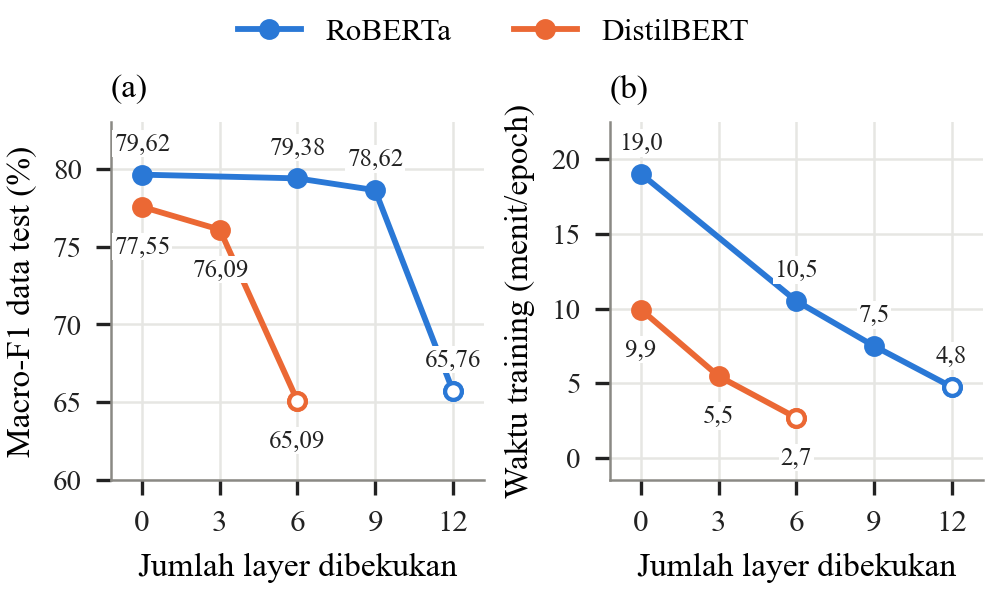
\includegraphics[width=\columnwidth]{fig_layer_dibekukan}
\caption{Pengaruh jumlah layer yang dibekukan pada early fusion terhadap (a) macro-F1 data uji dan (b) waktu training per epoch. Titik kosong menandai model yang seluruh layernya dibekukan (satu seed); titik lain adalah rata-rata tiga seed.}
\label{fig:frozen}
\end{figure}

\subsection{Pengaruh Parent Comment}
Friedman test menunjukkan bahwa ketiga input menghasilkan macro-F1 yang berbeda ($p = 0{,}009$, Kendall's $W = 0{,}78$). Gambar~\ref{fig:input} menunjukkan bahwa parent menaikkan macro-F1 kedua model. Early fusion menaikkan macro-F1 sebesar 1,10 poin pada RoBERTa dan 0,69 poin pada DistilBERT, sedangkan late fusion menaikkan 0,78 dan 0,72 poin. Keempat kenaikan signifikan menurut paired t-test setelah koreksi Holm dan menurut McNemar. Biaya early fusion kecil, karena waktu training hanya bertambah 1,15--1,16 kali dan latensi batch 1 serta memori praktis tidak berubah, meskipun latensi per contoh pada batch 32 menjadi sekitar dua kali lipat.

\begin{figure}[t]
\centering
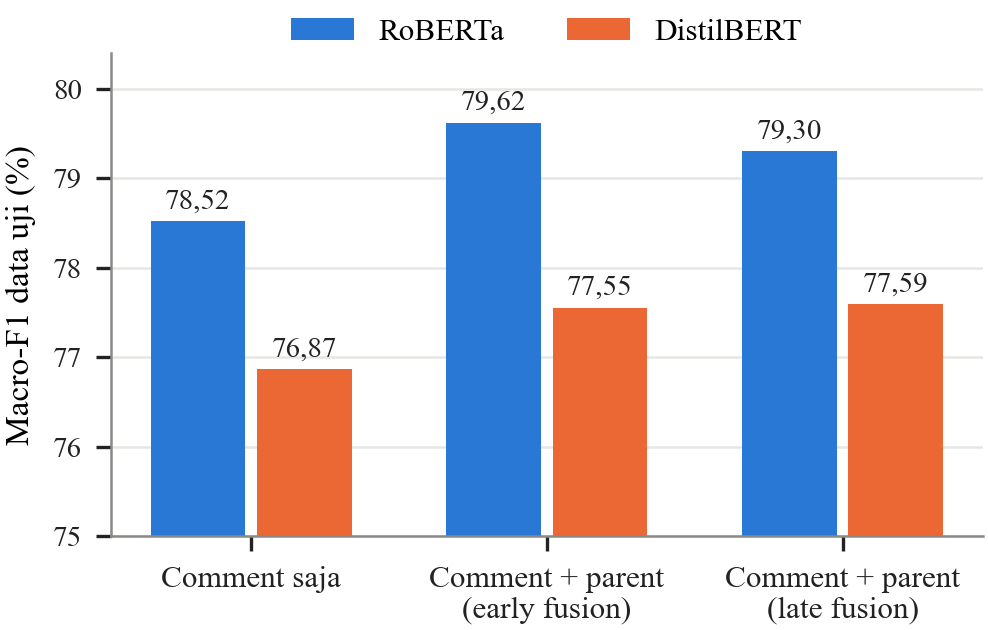
\includegraphics[width=\columnwidth]{fig_macro_f1_input}
\caption{Macro-F1 data uji untuk setiap model dan konfigurasi input (rata-rata tiga seed). Sumbu vertikal dimulai dari 75\% agar selisih antarkonfigurasi terlihat.}
\label{fig:input}
\end{figure}

Manfaat parent tidak merata. Pada 10.737 comment yang membuat model comment saja RoBERTa ragu, early fusion menaikkan macro-F1 RoBERTa sebesar 8,18 poin, sedangkan pada comment yang sudah diprediksi dengan yakin hanya 0,25 poin. Kenaikan juga lebih besar pada comment 1--3 kata (2,59 poin) daripada comment lebih dari 10 kata (0,71 poin), dan mencapai 2,73 poin pada 593 comment yang muncul dengan label berbeda. Namun, parent juga dapat menyesatkan, karena pada RoBERTa parent memperbaiki rata-rata 6.236 prediksi per seed tetapi juga merusak 5.119 prediksi.

\subsection{Strategi Fusion Terbaik}
Early fusion memberikan macro-F1 tertinggi pada RoBERTa dan unggul 0,32 poin atas late fusion (CI 95\% 0,15--0,49, $p_{\mathrm{Holm}} = 0{,}023$, juga signifikan menurut McNemar). Pada DistilBERT, kedua strategi setara (77,55\% dan 77,59\%). Jika kedua model digabung, keunggulan early fusion belum signifikan ($p_{\mathrm{Holm}} = 0{,}158$, CI 95\% $-0{,}08$--0,36). Late fusion juga yang paling mahal, dengan waktu training sekitar 1,5 kali, memori 1,62--1,64 kali, dan latensi batch 1 1,70--1,79 kali early fusion.

\section{Pembahasan}

\subsection{Trade-off antara RoBERTa dan DistilBERT}
Hasil uji memberikan bukti statistik bahwa RoBERTa lebih akurat, tetapi selisihnya hanya 1,65--2,07 poin, sedangkan biayanya sekitar dua kali DistilBERT. DistilBERT mempertahankan sekitar 97--98\% macro-F1 RoBERTa dengan sekitar separuh sumber daya. Rasio biaya ini hampir sama pada ketiga input, sehingga kemungkinan besar ditentukan oleh ukuran model. RoBERTa lebih sesuai ketika akurasi menjadi prioritas dan sumber daya mencukupi, misalnya untuk analisis offline. DistilBERT lebih sesuai ketika latensi dan memori terbatas, misalnya pada alat moderasi yang memproses comment secara terus-menerus.

\subsection{Pembekuan Layer dan Distilasi}
Hasil uji mendukung bahwa jumlah layer yang dibekukan berpengaruh terhadap performa, tetapi pengaruhnya tidak linear. Pada RoBERTa, membekukan separuh layer hanya menurunkan macro-F1 sebesar 0,24 poin, yang terlalu kecil untuk dibedakan dari variasi sampel pada setiap seed, padahal waktu training dan memori berkurang hampir separuh. Penurunan baru terlihat jelas pada 9 layer dan menjadi drastis bila semua layer dibekukan, sehingga representasi pralatih tetap perlu di-fine-tune. DistilBERT lebih cepat kehilangan performa, kemungkinan karena layernya lebih sedikit. Pembekuan dan distilasi juga menghemat hal yang berbeda. Pembekuan hanya menghemat training, sehingga cocok bila model perlu sering dilatih ulang, sedangkan DistilBERT menghemat inferensi karena latensinya sekitar separuh RoBERTa.

\subsection{Peran Parent Comment}
Terdapat bukti statistik bahwa parent comment meningkatkan performa kedua model, meskipun rata-rata kenaikannya hanya sekitar satu poin. Hal ini wajar karena sebagian besar comment sudah dapat dipahami dari isinya sendiri. Parent menjadi penentu ketika comment ambigu. Balasan ``;)'', misalnya, muncul 68 kali di data uji dan hanya enam yang sarkas. Saat membalas ``Sarcasm doesn't translate well through text. Haha'', balasan ini sarkas, tetapi saat membalas ``What is your Guilty Pleasure?'', balasan yang sama tidak sarkas. Tanpa parent, model terpaksa memberikan prediksi yang sama untuk keduanya. Kenaikan ini jauh lebih kecil daripada laporan Dubey dkk.\ (7,1 poin \cite{dubey2026efficient} dan 6,8 poin \cite{dubey2025unpacking}), yang memakai subset 7.370 sampel dengan tanda baca dan huruf kapital dihapus. Model comment saja tanpa tanda baca mungkin lebih bergantung pada parent, meskipun dugaan ini belum diuji di sini.

\subsection{Early Fusion dan Late Fusion}
Early fusion menjadi strategi terbaik pada penelitian ini karena memiliki bukti statistik lebih akurat pada RoBERTa, tidak berbeda nyata pada DistilBERT, dan jauh lebih murah. Pada early fusion, token comment dapat memperhatikan kata tertentu di parent pada setiap layer, sedangkan pada late fusion kedua teks diringkas menjadi satu vektor terlebih dahulu dan baru bertemu di head klasifikasi. Karena makna sarkasme sering bergantung pada frasa tertentu di parent, cara late fusion tampaknya kurang menguntungkan. Late fusion mungkin tetap berguna bila satu parent dibalas banyak comment, karena vektor parent cukup dihitung sekali, tetapi skenario ini tidak diuji.

\subsection{Perbandingan dengan Penelitian Lain dan Keterbatasan}
Skor yang lebih tinggi pernah dilaporkan, misalnya F1 95,6\% pada \cite{dubey2026efficient} dan 0,917 pada \cite{zhang2025enhancing}, tetapi ukuran data, prapemrosesan, dan protokol evaluasinya berbeda. Potongan ``/s'' yang dibahas pada Bagian~II-A juga mungkin berperan, karena hampir semuanya berlabel sarkas dan tidak ada laporan yang dirujuk yang menyebutkan apakah potongan itu dibuang. Rasio biaya justru sejalan, karena RoBERTa pada \cite{dubey2026efficient} membutuhkan waktu training 1,76 kali DistilBERT.

Hasil uji tersebut mendukung jawaban ketiga pertanyaan penelitian, tetapi hanya berlaku pada dataset, pengaturan, dan tiga seed yang digunakan. Penelitian ini juga memiliki beberapa keterbatasan. Training dibatasi tiga epoch, padahal 24 dari 29 run final mencapai skor validasi terbaik pada epoch terakhir. Hanya satu dataset yang digunakan, dan labelnya berasal dari penanda ``/s'' sehingga comment sarkas tanpa penanda tercatat sebagai bukan sarkas \cite{khodak2018sarc}. Split uji resmi SARC tidak dapat digunakan karena teksnya tidak tersedia. Model yang dibekukan memakai learning rate dari fine-tuning penuh, model yang seluruh layernya dibekukan hanya memiliki satu seed, dan uji per konfigurasi hanya memiliki tiga pasangan. Selain itu, large language model tidak disertakan, dan semua angka efisiensi diukur pada satu GPU.

\section{Kesimpulan}

\nocite{*}
\bibliographystyle{IEEEtran}
\bibliography{references}

\end{document}
